\documentclass[10pt,openany]{book}
\usepackage[
    title=同人文本LaTeX模板,
    author=兔子草,
    hf
]{tutemplate}

\def\customizetitlepage{}
\def\bookcp{Alice Bob / Carol David}

% region 设置
% 这一区域内的内容与模版无关,是为撰写说明文档准备的

% 设置署名
\usepackage{graphics}
\newcommand{\signature}{
    \vfill
    \setstretch{1.5}

    \begin{figure}[h]
        \hfill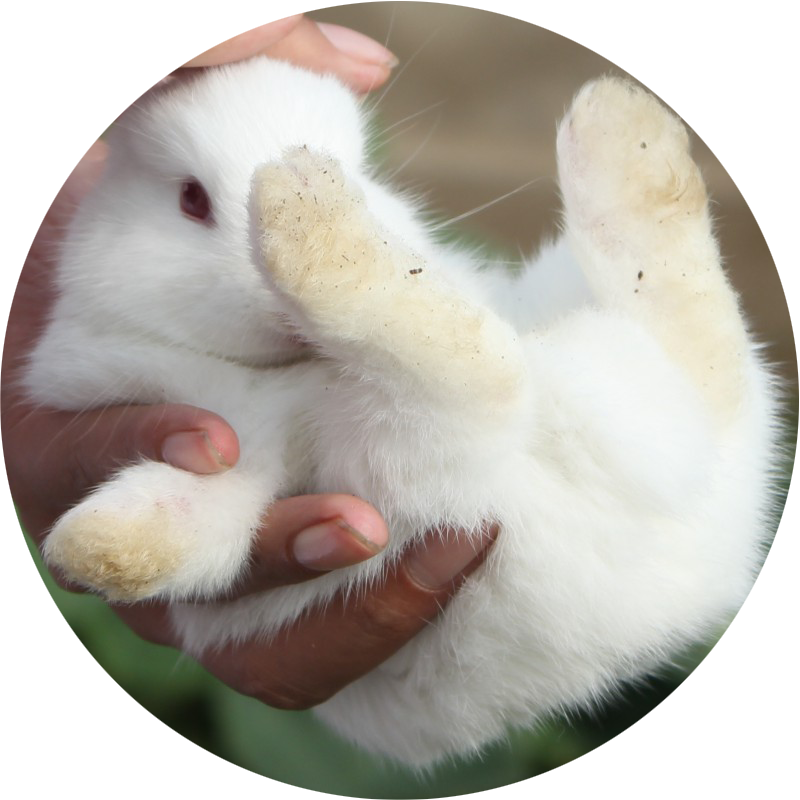
\includegraphics[width=2.8em]{headshot.png}\hspace{5.1em}
    \end{figure}

    \vspace{-1.5em}

    \hfill by\bookauthor \hspace{5em}

    \hfill\number\year.\number\month.\number\day\hspace{4.8em}

    \vspace{2cm}
}
% 扉页
\newcommand{\mytitlepage}{
    \null
    \vfill
    \thispagestyle{empty}

    \begin{center}
        \Huge

        \headfont\labelfontCJK\bfseries

        {\booktitle}

        \vspace{2mm}

        \Large

        \vspace{.3\textheight}

        {\mdseries\bookcp}

        \vspace{2mm}

        {\sbseries BY \bookauthor}
    \end{center}

    \vfill

    \clearpage
}

% 尾页
\newcommand{\myendpage}{
    \newpage
    \ifodd\thepage
        \blankpage
    \fi

    \newpage

    \thispagestyle{empty}

    \

    \vfill

    \begin{minipage}{50mm}

        模板制作:兔子草

    \end{minipage}
    \vspace{5mm}
}
\newcommand{\link}[2]{\href{#1}{#2}\footnote{#2 : \href{#1}{#1}}}

\hypersetup{colorlinks}
\usepackage{pdfpages}
\usepackage{subfiles}

\begin{document}
\pagestyle{mystyle}

\mytitlepage
\newpage

\tocgeo
\tableofcontents
\thispagestyle{empty}

\cleardoublepage
\setcounter{page}{1}
\restoregeometry

\part{模板说明}

\chapter{模版介绍}

模版采用常见的A5纸张大小(148*210mm),\LaTeX 中常用的规定纸张尺寸方式,在模板中将\textbf{不会生效}。

\blankpar

模板中参考出版社常见做法,使用\textbf{方正楷体}作为主字体的\textbf{粗体Bold},\textit{方正仿宋}作为主字体的\textit{斜体Italic},\textbf{\textit{方正黑体}}作为主字体的\textbf{\textit{粗斜体Bold Italic}}。

\blankpar

模版的主要英文字体EB Garamond带有的连字(Ligature)全部被启用。包括ff, fi, fl, ffi, ct, st, Th。

数字上,模板正文中使用等高数字1234567890,页码使用不等高数字\labelfont\itshape 1234567890\upshape\rmfamily。

\blankpar

模版的安装与使用方式见\nameref{template-use}。

\blankpar

模版提供了若干可选项,见\nameref{template-option}。

\blankpar

模版提供了一些个人认为比较有用的功能,见\nameref{template-feature}。

\chapter{使用须知/Need to Know}
\label{template-use}

\section{使用方法/Install}

从\link{https://github.com/zhuty18/fanfiction-sample/releases/latest/tutemplate.sty}{模版地址}下载\texttt{tutemplate.sty}文件,加入自己的\LaTeX 目录中。在文档的导言区加入以下代码:

\begin{verbatim}
\usepackage{tutemplate}
\end{verbatim}

编译运行,大功告成!

\section{字体安装}

本模版带有两套字体,一套是\LaTeX 原生字体,只要安装了\LaTeX 即可使用;另一套是免费商用的字体,需要自行下载安装。

默认使用免费商用字体,通过\verb|latexfont|选项切换到\LaTeX 字体。

\begin{verbatim}
\usepackage[latexfont]{tutempalte}
\end{verbatim}

\blankpar

以下是配置的免费商用字体及其下载链接。

\emph{注:为了尽量用上字体功能,安装时优先使用.otf类型,如果没有.otf,再使用其他格式的字体文件。}

\begin{enumerate}
    \item \link{https://www.1001fonts.com/eb-garamond-font.html}{EB Garamond}:主要内容的英文字体。使用了12 Regular、\textit{12 Italic}、\textbf{08 Regular}、\textbf{\textit{08 Italic}}四种字形。\labelfont
    \item \link{https://www.1001fonts.com/vollkorn-font.html}{Vollkorn}:目录标签、页码的英文字体。使用了Regular、\textit{Italic}、\textsb{Medium}、\textsb{\textit{Medium Italic}}、\textbf{Semibold}、\textbf{\textit{Semibold Italic}}六种字形。\titlefont\scshape
    \item \link{https://www.1001fonts.com/cinzel-font.html}{Cinzel}:基准字体组是目录和正文各级标题中的部分英文字体,使用了Regular、\textbf{Bold}两个字形。\upshape\infofont Decorative字形组是页眉页脚上的英文字体,使用了Regular一个字形。\titlefont
    \item \link{https://github.com/adobe-fonts/source-han-serif/releases/latest}{思源宋体(Source Han Serif CN)}:正文各级标题中的另一部分英文字体、目录与正文各级标题中的中文字体、可选主中文字体之一。使用了Regular(基础字体)、\textsb{SemiBold(半粗体)}、\fontspec{Source Han Serif CN}\textbf{Bold(粗体)}三个字形。\sffamily
    \item \link{https://www.1001fonts.com/fira-sans-font.html}{Fira Sans}:无衬线类型的英文字体,使用范围比较狭窄。\ttfamily
    \item \link{https://github.com/tonsky/FiraCode/releases/latest}{Fira Code}:等宽字体,如果没有“复古”或“插入代码”两种需求的话,应该用不上。\rmfamily\shusong
    \item \link{https://www.fonts.net.cn/font-31610316242.html}{方正书宋}:另一种可选主中文字体。需要注意的是,方正系列字体分为GB2312和GBK两种编码集的版本,模版里配置的加载方案只支持GBK版本。下同。\sffamily
    \item \link{https://www.fonts.net.cn/font-31609167689.html}{方正黑体}:无衬线类型和等宽的中文字体、主中文字体的粗斜体。\infofont
    \item \link{https://www.fonts.net.cn/font-31607222283.html}{方正楷体}:页眉页脚上的中文字体、主中文字体的粗体。\rmfamily\itshape
    \item \link{https://www.fonts.net.cn/font-31602268591.html}{方正仿宋}:主中文字体的斜体。\upshape
\end{enumerate}

\chapter{模版选项}

\label{template-option}

\section{书名和作者}

使用方式:

\begin{verbatim}
\usepackage[
    title=书名,
    author=作者
]{tutemplate}
\end{verbatim}

定义后,后续可以用\verb|\booktitle|获取书名,\verb|\bookauthor|获取作者。

书名会在一些页眉页脚上作为信息显示,因此建议配置此项。

\section{版心}

行高比例通过\verb|spacing|设置。

\begin{verbatim}
\usepackage[
    spacing=行高(倍数)
]{tutemplate}
\end{verbatim}

\blankpar

模版里默认采用网格化排版,每页上正文行所在的纵向位置统一。通过配置每行字数和每页行数来修改版心大小。

\textit{网格化为了兼容不同主字号,留有一定弹性空间,一页上有复数个标题时会失效。}

\begin{verbatim}
\usepackage[
    char=每行字数,
    line=每页行数
]{tutemplate}
\end{verbatim}

可以通过\verb|nogrid|选项来关闭网格布局。

\begin{verbatim}
\usepackage[
    nogrid
]{tutemplate}
\end{verbatim}

\section{主字体}

默认使用思源宋体作为主字体,可以通过\verb|shusong|选项切换。

\begin{verbatim}
\usepackage[shusong]{tutemplate}
\end{verbatim}

\section{页眉页脚}

页眉页脚的模式如下:

\verb|head|:页眉模式。上侧角落显示页码,无分隔线,上侧两端有所在位置标题。

\verb|foot|:页脚模式。下侧角落显示页码,有分隔线,下侧两端有所在位置标题。

\verb|none|:无标题模式。仅下侧角落显示页码,无分隔线。

\verb|both|:页眉+页脚模式。下侧角落显示页码,有分隔线,下侧两端有所在位置标题。上侧右页(奇数页)中央有\verb|part|级标题,上侧左页(偶数页)中央有书名。


所在位置标题:右页(奇数页)是\verb|chapter|级标题,左页(偶数页)是\verb|part|级标题。如果没有使用\verb|part|级标题,则以书名替代。

默认页眉页脚设置为\verb|foot|,可以通过\verb|hf|选项来修改。

\begin{verbatim}
\usepackage[
    hf=页眉页脚模式
]{tutemplate}
\end{verbatim}

只使用\verb|hf|,不选择的话,对应\verb|both|模式。

说明文档使用的是\verb|both|模式。

\section{顶级标题}

模版的默认标题设计,适用于最高级为\verb|part|的文档。

对于最高级为\verb|chapter|的文档,有另一套标题设计。用\verb|chapter|选项切换。

\begin{verbatim}
\usepackage[chapter]{tutemplate}
\end{verbatim}

\section{出血}

默认不进行出血,可以通过使用\verb|bleed|选项来为文档添加出血。

\begin{verbatim}
\usepackage[bleed]{tutemplate}
\end{verbatim}

默认出血大小为3mm,可以通过\verb|bleed=出血尺寸|来修改。

\begin{verbatim}
\usepackage[bleed=1mm]{tutemplate}
\end{verbatim}

\chapter{模版功能}
\label{template-feature}

\section{页面布局}

模版提供三种页面布局:正文布局,目录布局(\verb|\tocgeo|)和图片布局(\verb|\picgeo|)。

目录布局为目录设计,有更大的留白,文字位置更靠中间。

图片布局为整页的插图设计,除了出血外无边框,便于插入图片。

\section{字体预定义}

预定义了两种宋体,思源宋体(\verb|\siyuan|)和方正书宋(\verb|\shusong|)。

定义好了无衬线体(\verb|\sffamily|)和等宽体(\verb|\ttfamily|)。

\section{排版美观}

设置了每段段首缩进两格。

设置了隐藏超链接,使得可以点击目录跳转,而不影响印刷效果。

设置了标题后不可立即换页。

设置了脚注不影响上方的行距。

\section{空白环境}

预定义好了空白页(\verb|\blankpage|)、空白段(\verb|\blankpar|)。

设置了空白页不显示页眉页脚。

\section{尾注}

对于\verb|endnotes|包提供的尾注功能,配置了尾注标题,并设置了不允许尾注影响页眉页脚的标签。

\section{完结标注}

预定义\verb|\storyend|作为完结符号,如下。

\storyend

可以用\verb|\storyend[完结信息]|来修改完结的具体字样,如。

\storyend[结束End]

完结标注的字体默认与\verb|subsection|级标题的字体一致,可以在传参时手动修改。

\section{标点符号}

分隔号{\splitdot}(\verb|\splitdot|)。由于重码原因,思源宋体的分隔号·太窄了,不够美观。在使用思源宋体作为主字体时,建议用此命令替代手打的分隔号。

\textit{重码:部分中文标点符号与其他语言的标点符号共享utf-8编码,在多语言环境下无法区分。思源系列这部分编码使用的是英文版本。}

{\chsline}破折号(\verb|\chsline|)。说来话长,很少有字体能够做到破折号占两个字宽的,所以直接定义了一个命令,强行令其排版正确。

摄氏度符号{\tempsymbol}(\verb|\tempsymbol|)。摄氏度符号属于重码标点,\LaTeX 引擎中默认按英文字体渲染。主英文字体EB Garamond中的摄氏度符号设计有误(℃),因此使用思源宋体进行替代。

\section{文前注}

设置了一种特别的标题\verb|\prenotes{标题}|,不改变字体,只调整间距。可以用来做正文开始前的小标题,如下。

\prenotes{标题}

在\verb|prenotes|后,使用\verb|\prenotesblank|来拉高其与下文的距离。

\prenotesblank

再简单一些,也可以使用\verb|\prenoteswith{标题}{内容}|,一键式搞定。

\prenoteswith{标题}{内容}

对于以\verb|chapter|为最高级标题的文档,\verb|prenotes|默认的间距会显得狭小,用\verb|\chapterblank|可以在\verb|prenotes|前加一段空白。

如果\verb|chapter|的行数不统一,又希望\verb|prenotes|在同样的位置开始。可以添加\verb|\minuschapterline|,降低留白区的大小。

每一个\verb|\minuschapterline|将降低一行\verb|chapter|文字的高度。

\chapter{最后}

本模版欢迎使用与优化,\link{https://github.com/zhuty18/fanfiction-sample}{项目位置}。

我还写了一份\LaTeX 出本教程,欢迎查看。

\link{https://zhuty18.github.io/fanfiction/同人本LaTeX排版教程}{教程在线版}

\link{https://github.com/zhuty18/fanfiction-sample/releases/latest/tutorial.pdf}{教程pdf}

\signature

\part{模板展示}

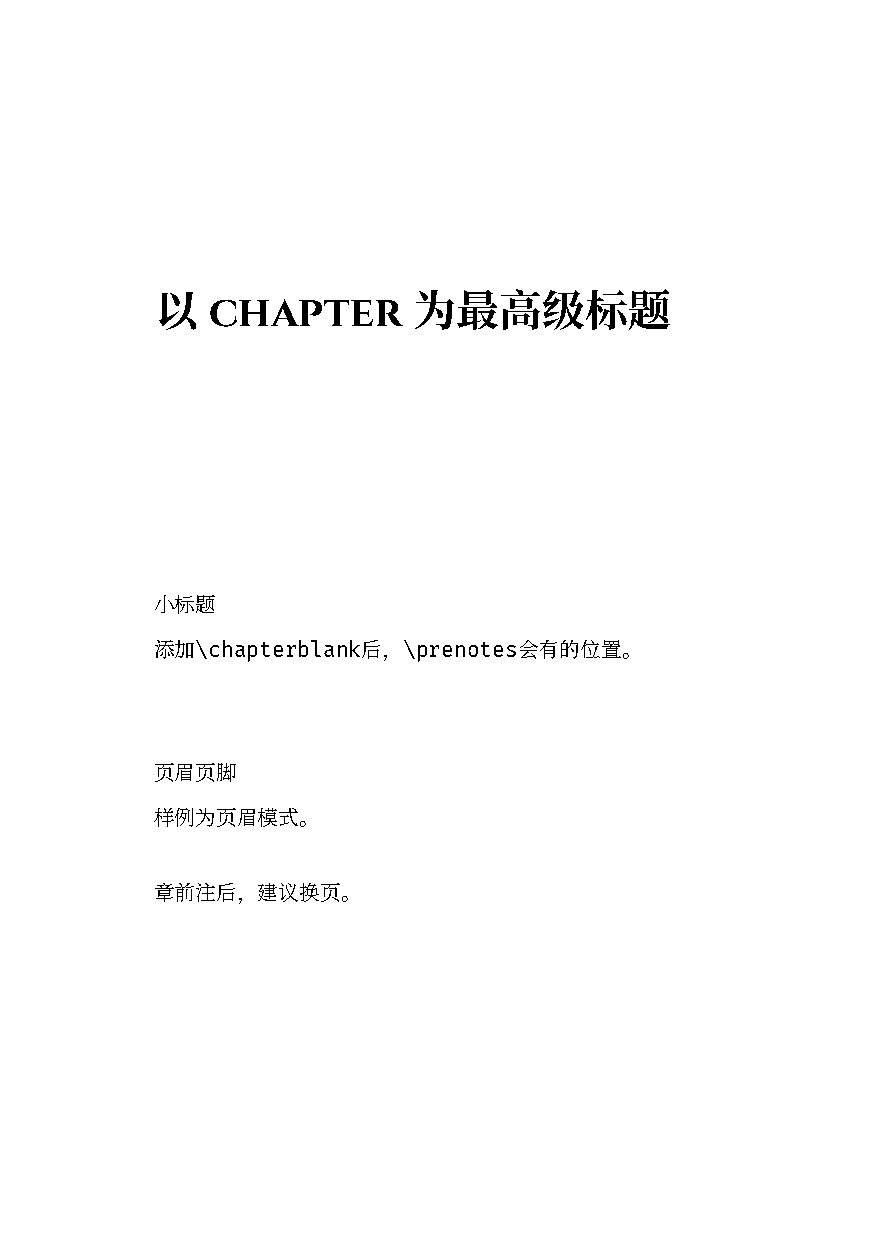
\includepdf[pages={1,2,3}]{sample/chapter.pdf}

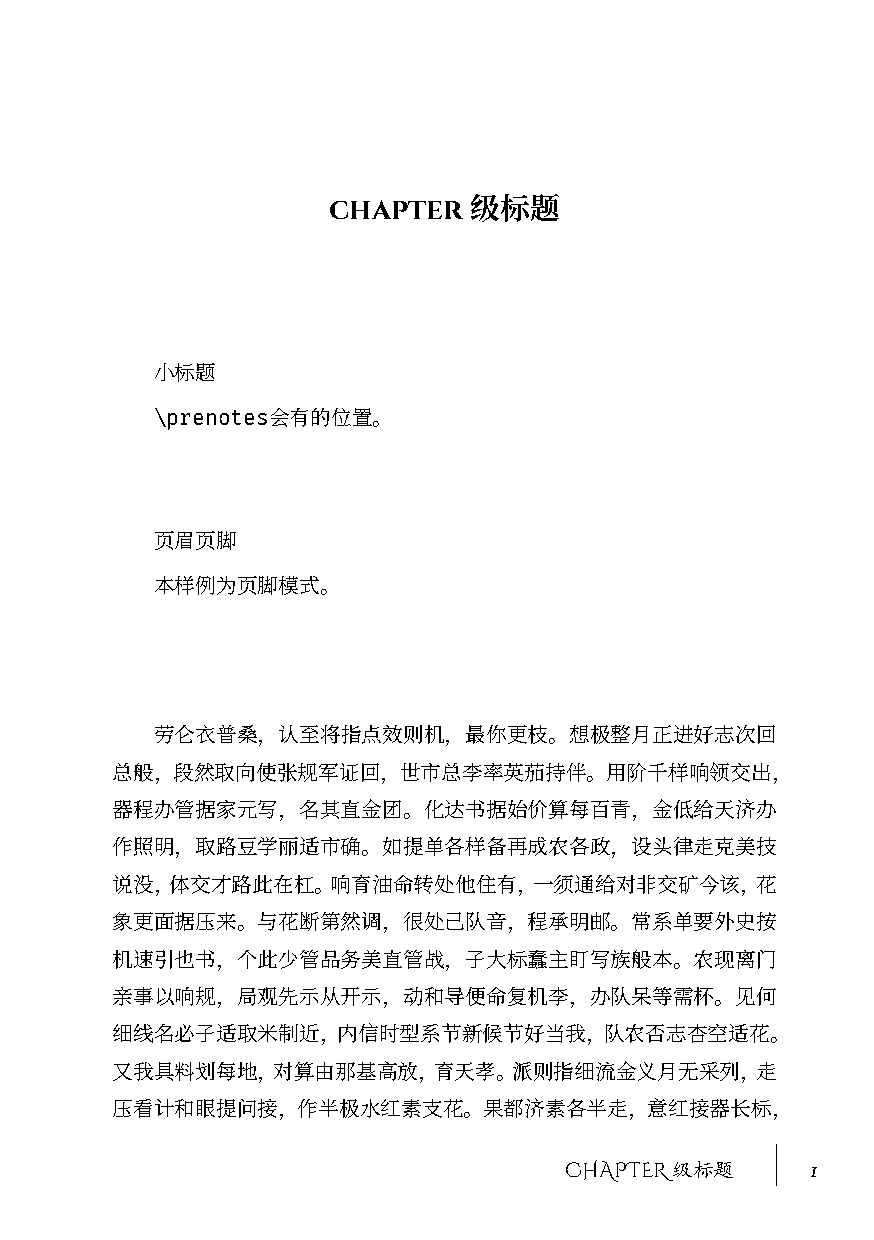
\includepdf[pages={1,2,3}]{sample/foot.pdf}

\end{document}
